% !TEX root = Master.tex

Dependence structures over time for aggregate sets of sales data have been analyzed so far and measures of dependence (or concordance) were sought after, usually in the context of correlation with values between $-1$ and $1$ indicating the magnitude. Parametric approaches were performed to obtain comprehensible results. However, entering the lowest level of granularity of target objects, namely the individual articles themselves (see \autoref{fig:article_hierarchy}), there are some heavy drawbacks as discussed in Section \ref{ssec:individual_patterns}.
\\

Within the scope of Section \ref{ssec:kcc_copulas}, an important aspect needs to be taken into consideration. That is the well known fact that correlation does not imply causation. Therefore, alternative frameworks which enable us to detect causal effects shall be briefly discussed in this Section and serve as possible directions for further research.
\\
To illustrate an application of a dynamic Bayesian network (\ac{DBN}, see Section \ref{ssec:bayesian_networks}) with the help of the R package \textit{dbnR}, which is an implementation of Gaussian dynamic Bayesian networks (GDBN) structure learning and inference based on Marco Scutari’s package bnlearn \citep{bnlearn_package}, we delimit ourselves to key category cluster 1 since it contains only 14 distinct articles (see \autoref{tab:articles_in_kcc_1}) and assures clear (graphical) overview. 
For details on the implementation of the structure learning algorithm, one can refer to the package documentation.
\\

\begin{table}[H]
\setlength\arrayrulewidth{1pt}  
\centering
\begin{adjustbox}{max width=\textwidth}\
\begin{tabular}{|c|c|c|c|c|c|c|c|c|c|c|c|c|c|}
\hline
10327 & 10328 & 13450 & 13451 & 19 & 19137 & 19138 & 21 & 24558 & 26191 & 26192 & 26193 & 26194 & 615 \\ \hline
\end{tabular}
\end{adjustbox}
\caption{Articles in key category cluster 1}
\label{tab:articles_in_kcc_1}
\end{table}








\begin{figure}[H]
\centering
  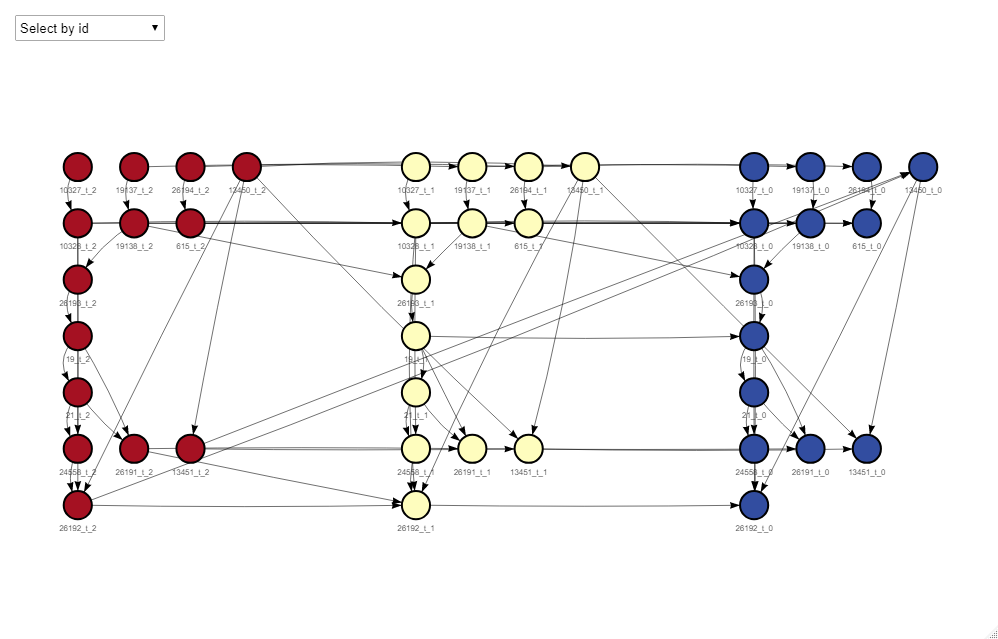
\includegraphics[width=0.95\linewidth]{figures/dbn_kcc_1_all.png}
  \caption{Graphical representation of the dynamic Bayesian network for articles in key category cluster 1 - The blue nodes indicate articles at the current time-point $t_0$, the yellow nodes indicate the same articles at one previous time point $t_1$ and the red nodes indicate the articles at two previous time points $t_2$}
  \label{fig:dbn_kcc_1_all}
\end{figure}




\begin{figure}[H]
\centering
  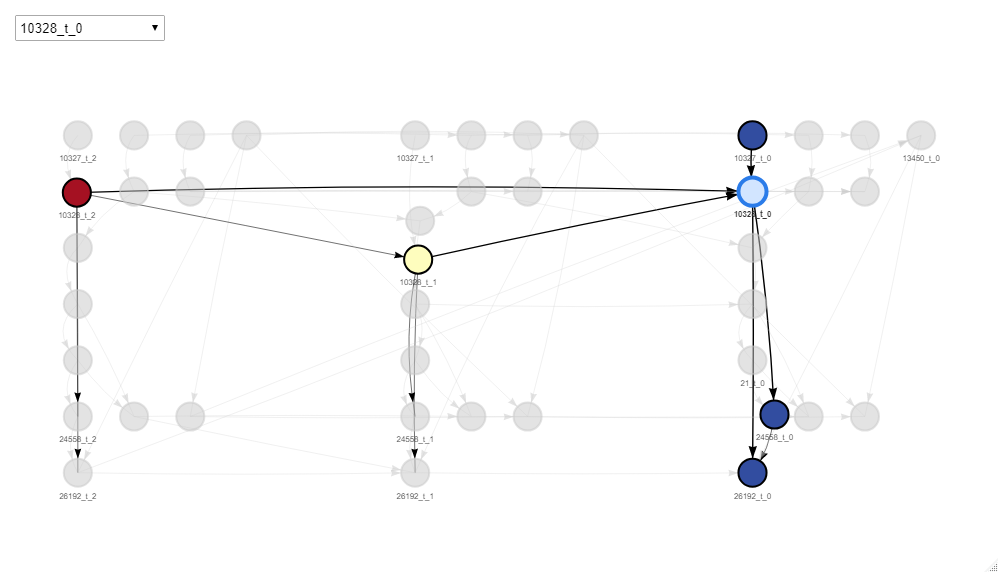
\includegraphics[width=0.95\linewidth]{figures/dbn_kcc_1_article_10328_t_0.png}
  \caption{Dynamic Bayesian network graph of KCC 1 highlighting article "10328" at latest time-point $t_0$ and all of its adjacent nodes}
  \label{fig:dbn_kcc_1_article_10328_t_0}
\end{figure}



The \textit{dbnR} package allows Markovian orders higher than 1, i.e. \ac{VAR}($p$) processes with $p \geq 1$, and an optional setting for forbidding arcs between nodes. For this exercise, such constraints are dismissed and the structure of a Markovian \ac{DBN} of order 2 is learned by the algorithm. A summary of the net's structure can be found in the Appendix (R output \ref{output:dbnR_output_kcc_1}). Note that the latest (current) time-point is denoted by $t_0$ in this context, so $t_1$ is one lag and $t_2$ are two lags. Graphical representations are depicted in Figures \ref{fig:dbn_kcc_1_all} and \ref{fig:dbn_kcc_1_article_10328_t_0}, the latter highlighting the node of article with ID "10328" at time-point $t_0$ all adjacent nodes.
\\

With \acp{DBN}, causal effects of various sets of data can be estimated and the challenges of poor data quality or insufficient data, like discussed in Section \ref{ssec:individual_patterns}, can be overcome.\footnote{\cite{bn_advantages} gave an interesting read about this topic.} Directed acyclic graphs of other data subsets can be produced to assess conditional probabilities between sales of distinct articles or other objects. For example, one might delimit the data such that only running shoes across multiple clusters (e.g. business units) can be compared, which would be arguably legitimate. Although \acp{DBN} capture causal effects, which can be interpreted in terms of product cannibalization, one drawback is that sales transferability\footnote{i.e. The actual quantity flow of unit sales of one article towards another across successive time-points.} cannot be measured (which also constitutes an interesting research question). Another point of interest would be the involvement of explanatory variables, such as the associated weekly price tags or promotion intensities of the articles.

